\documentclass{article}
\usepackage{pdfpages}
\usepackage{graphicx}  % For PNG
\usepackage[left=2cm, right=2cm, top=2cm]{geometry}
\usepackage[newfloat]{minted}
\usepackage{enumitem}
\usepackage{amsmath}    % For bmatrix
% Give Table of Contents Hyperlinks
\usepackage{hyperref}
\hypersetup{
    colorlinks,
    citecolor=black,
    filecolor=black,
    linkcolor=black,
    urlcolor=blue
}
\newcommand\ddfrac[2]{\frac{\displaystyle #1}{\displaystyle #2}}
% \renewcommand{\theenumi}{\Alph{enumi}} % https://tex.stackexchange.com/a/2292

\pagenumbering{gobble}
% \pagenumbering{roman} % set the numbering style to lowercase letter

\title{\textbf{Homework 5}}

\author{MacMillan, Kyle}
\date{November 26, 2018}

\begin{document}


\addcontentsline{toc}{section}{Title}
\maketitle

\newpage
\tableofcontents
\addcontentsline{toc}{section}{Table of Contents}
\newpage
\listoffigures
\addcontentsline{toc}{section}{List of Figures}

\pagenumbering{roman}   % Set TOC page numbering to lowercase roman numerals


%%%%%%%%%%%%%%%%%%%%%%%%%%%% INTRO SECTION %%%%%%%%%%%%%%%%%%%%%%%%%%%%
\newpage
\hypersetup{
    colorlinks,
    citecolor=blue,
    filecolor=black,
    linkcolor=blue,
    urlcolor=blue
}
\pagenumbering{arabic}  % Set content page numbering to arabic numerals

\setcounter{page}{1}
\newpage
\section{\textbf{Chapter 11}}
\subsection{Problem 3}
To complete this problem I created a class to generate a random map of any 
size you want up to 99. It generates a random number of obstacles of random 
size. Play around with it, it's fun. You can change the random numbers or just 
run the file multiple times. Code for this problem can be found 
\href{https://github.com/macattackftw/RoboticsHW/blob/master/HW5/problem11_3.py}{here}.

Demonstration is shown in Figure \ref{fig:p11_3_1}. This is an application of 
the WaveFront BFS algorithm. From there it goes on to find the shortest path as 
seen in Figure \ref{fig:p11_3_2}. The seed for that particular example 
is: \texttt{7635686187880284248}

\begin{figure}[h]
    \centering
    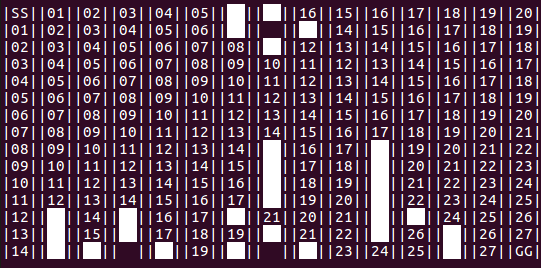
\includegraphics[scale=2.5]{problem11_3_1}
    \caption{WaveFront Distance Evaluation}
    \label{fig:p11_3_1}
\end{figure}

\begin{figure}[h]
    \centering
    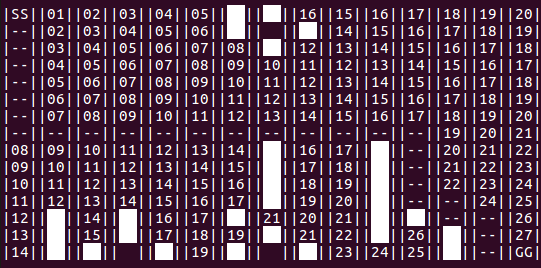
\includegraphics[scale=2.5]{problem11_3_2}
    \caption{WaveFront Shortest Path}
    \label{fig:p11_3_2}
\end{figure}

I discussed the algorithm with Dr. McGough and he was in agreement that it 
didn't matter if you begin the wave at the start or goal. I reversed the point 
of origin for the WaveFront because it makes more sense in my brain. The result 
is the same so long as you start the WaveFront from one end and walk from the 
other end back to the WaveFront origin. It's more robust if done this way, that 
way if the goal is moving you don't have to redo the BFS, you just redo the 
navigation step.


\newpage
\section{\textbf{Chapter 16}}
\subsection{Problem 1}
Given mesaurements of: $z_1 = 284$, $z_2 = 257$, and $z_3 = 295$ and standard 
deviations of $\sigma_1 = 10$, $\sigma_2 = 20$, and $\sigma_3 = 15$ we can setup 
variance as the square of the standard deviations:

\begin{enumerate}
    \item 100
    \item 400
    \item 225
\end{enumerate}

Given the variance we can apply the formulas from section 16.3.3 in the book to 
obtain an estimated state $\^{x} = 282.90163934426226$. Code for this problem 
can be found 
\href{https://github.com/macattackftw/RoboticsHW/blob/master/HW5/problem16_1.py}{here} 
and in the code snippet \ref{code:16_1}.

\begin{code}
\label{code:16_1}
\begin{minted}{python}
    # Given values
    measured = np.array([284, 257, 295])
    std = np.array([10, 20, 15])

    # Calculate variance
    var = std * std

    # Sensor fusion to obtain x_hat
    top = 0.0
    bot = 0.0
    for i in range(3):
        top += (measured[i] / var[i])
        bot += 1 / var[i]

    # Estimated distance
    x_hat = top / bot
\end{minted}
\end{code}


\subsection{Problem 2}{\label{problem:16.2}}
Given 40 measurements at 2 meters we can calculate the mean:

\begin{enumerate}[label=\Alph*]
    \item 2.23521735
    \item 1.86443904
    \item 2.33806001
\end{enumerate}

That is how far off each senor averages from 2 meters. Each new sensor reading 
then has that mean subtracted from it to yield:

\begin{enumerate}[label=\Alph*]
    \item 2.22255225
    \item 2.03233526
    \item 1.79719609
\end{enumerate}

We can then apply the formula provided in the sensor fusion portion of the book 
for an expected distance, $\^{x} = 2.057449909256987$ meters. The code for 
this can be found 
\href{https://github.com/macattackftw/RoboticsHW/blob/master/HW5/problem16_2.py}{here} 
and in the code snippet \ref{code:16_2}.

\begin{code}
\label{code:16_2}
\begin{minted}{python}
    # Calculate mean and standard deviation
    mean = np.mean(dist_sens, dtype=np.float64, axis=0)
    std = np.std(dist_sens, dtype=np.float64, axis=0)

    # Reshape because it doesn't need to be 2D
    np.reshape(mean, (1, 3))
    np.reshape(std, (1, 3))

    # Input for this step
    new_sens = np.array([2.4577696, 1.8967743, 2.1352561]) + (2.0 - mean)

    # Calculate variance
    var = std * std

    # Sensor fusion to obtain x_hat
    top = 0.0
    bot = 0.0
    for i in range(3):
        top += (new_sens[i] / var[i])
        bot += 1 / var[i]

    # Estimated distance
    x_hat = top / bot
\end{minted}
\end{code}


\newpage
\section{\textbf{Chapter 17}}
\subsection{Problem 2}
% http://roboscience.org/book/html/AdvFiltering/KalmanFilters.html?#different-sensor-types
% If I have time, rewrite it to match this section...
The code for this problem can be found 
\href{https://github.com/macattackftw/RoboticsHW/blob/master/HW5/problem17_2.py}{here}.

The problem asked us to fuse three different measurements to determine an 
estimate of the covariance. To do that I first applied the same sensor fusion 
techniques utilized in \hyperref[problem:16.2]{Chapter 16, Problem 2}. This 
sensor fusion led to:

$$\^{x} = 10.557142857142857$$
$$\^{y} = 18.18695652173913$$
$$x_{var} = 0.02857142857142857$$
$$y_{var} = 0.03260869565217391$$

Which can also be seen in Figure \ref{fig:p17_2}. We can also find the mean of 
$x$ and $y$ given the three initial measurements and can use them to find the 
covariance using:

$$\ddfrac{\sum_{i=1}^{3} (\mu_x - x_i) * (\mu_y - y_i)}{3}$$

So putting it all together we end up with the covariance matrix:

\[
P =
  \begin{bmatrix}
    0.02857142857142857 & -0.1694444444444446 \\
    -0.1694444444444446 & 0.03260869565217391
  \end{bmatrix}
\]

\begin{figure}[h]
    \centering
    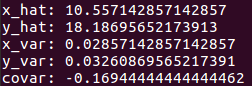
\includegraphics[scale=2.5]{problem17_2_data}
    \caption{Problem 17.2 Estimates}
    \label{fig:p17_2}
\end{figure}


\newpage
\subsection{Problem 3}
Lecture slide \href{https://d2l.sdbor.edu/content/enforced/2018FA/1139913-CENG-CSC-415-515-M001-2018FAIntroductiontoRobot/Robotics_Kalman.pdf}{58} is where I began for this problem. 

\textbf{Step 1}: Discretize

This is accomplished with the \href{https://en.wikipedia.org/wiki/Fundamental_theorem_of_calculus#Geometric_meaning}{Fundamental Theorem of Calculus}.

$$y_n = \frac{x_{n+1} - x_n}{0.1}$$
$$\frac{y_{n+1} - y_n}{0.1} = -cos(x_n) + 0.5sin(t_n)$$

\textbf{Step 2}: Solve for $n + 1$

This is done with some simple algebra to move the terms around.

$$x_{n+1} = x_n + 0.1y_n$$
$$y_{n+1} = y_n - 0.1cos(x_n) + 0.05sin(t_n)$$

\textbf{Step 3}: Partial derivatives

$$
\[
F =
  \begin{bmatrix}
    \frac{\partial}{\partial x} \big(x_n + 0.1y_n\big) & \frac{\partial}{\partial y} \big(x_n + 0.1y_n\big) \\
    \frac{\partial}{\partial x} \big(y_n - 0.1cos(x_n) + 0.05sin(t_n)\big) & \frac{\partial}{\partial y} \big(y_n - 0.1cos(x_n) + 0.05sin(t_n) \big)
  \end{bmatrix}
\]
$$

$$
\[
F =
  \begin{bmatrix}
    1.0 & 0.1 \\
    0.1sin(x_n) & 1.0
  \end{bmatrix}
\]
$$

Using those equations and matrices we can now apply the Extended Kalman Filter 
steps.

\begin{code}
\label{code:17_3}
\begin{minted}{python}
    # For each time step
    for i in range(N):
        # Predict State
        x_hat0 = updateXhat0(x_hat0[0][0], x_hat0[0][1], t[i]) + r[i]

        # Predict estimate covariance
        P = updateP0(V, updateF(x_hat0[0][0]), P)

        # Optimal Kalman gain
        K = updateK(H, P, W)

        # Update state estimate
        z = x_hat0[0][0] + q[i]
        x_hat1 = updateXhat1(x_hat0, K, z)

        # Update estimate covariance
        P = updateP1(np.identity(2), K, H, P)
\end{minted}
\end{code}

The code for \hyperref[code:17_3]{Chapter 17, Problem 3} shows the steps we take 
to obtain a filtered prediction. Figure \ref{fig:p17_3x} shows the $x$ component 
and Figure \ref{fig:p17_3y} shows the $y$ component. The $y$ component did not 
have an observation, so the prediction is not as close as the $x$ component. The 
function calls just perform the necessary procedure to complete that step of the 
Extended Kalman Filter. Code for this problem can be found 
\href{https://github.com/macattackftw/RoboticsHW/blob/master/HW5/problem17_3.py}{here}.

Also to note is that the filter predicts $y$ will follow in the general 
direction of $x$ since it had no observations in $y$.

\newpage

\begin{figure}[h]
    \centering
    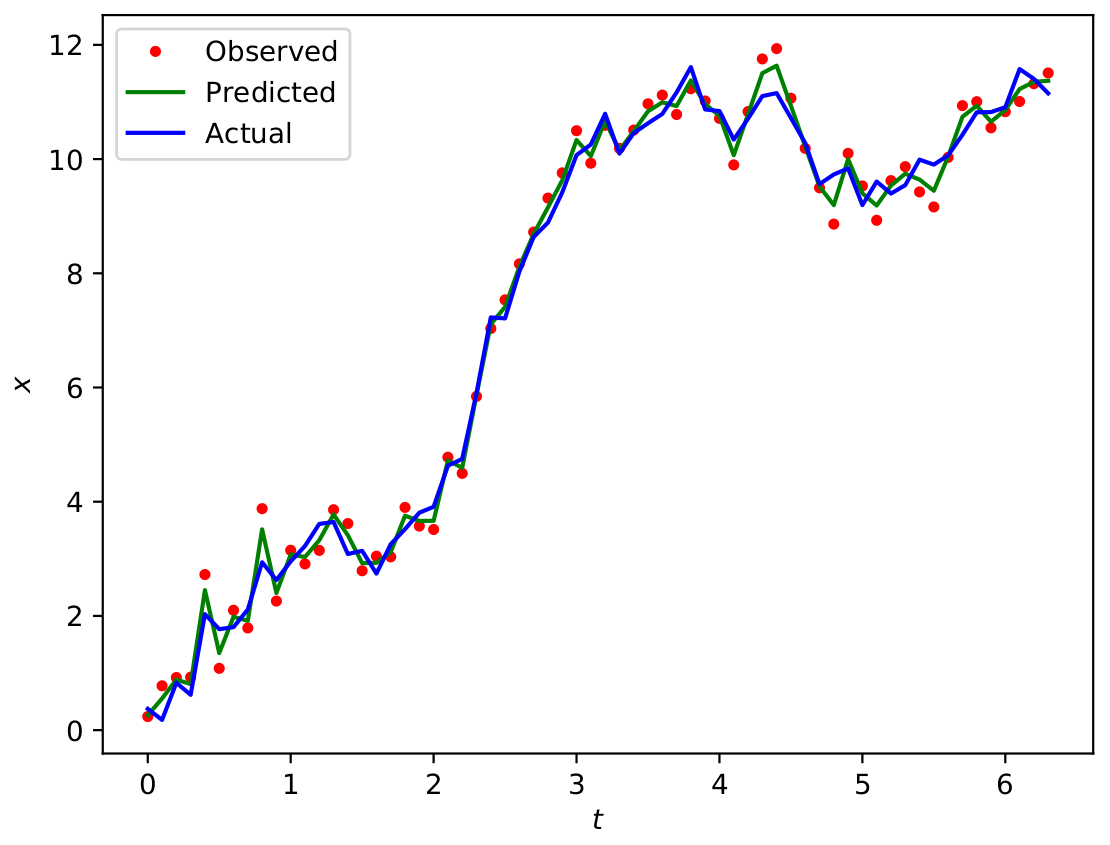
\includegraphics[scale=1]{problem17_3_x}
    \caption{Problem 17.3 Kalman Filtering 1}
    \label{fig:p17_3x}
\end{figure}

\begin{figure}[h]
    \centering
    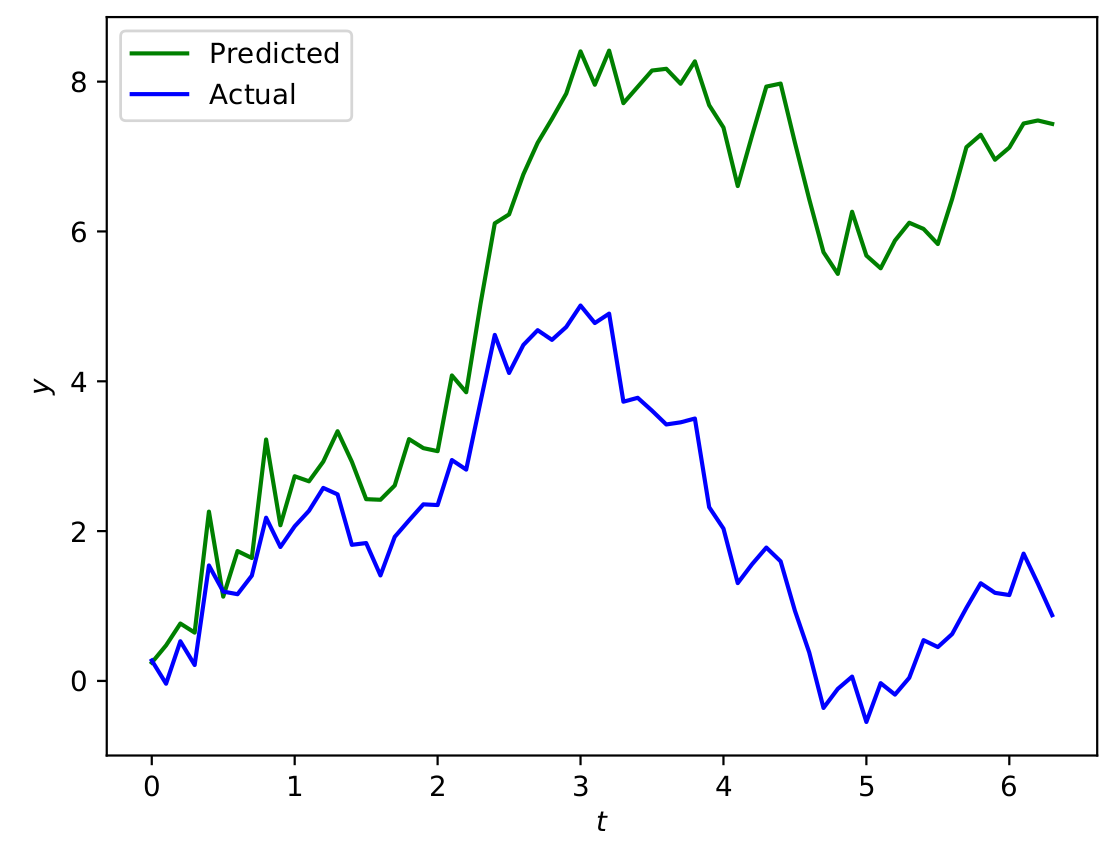
\includegraphics[scale=1]{problem17_3_y}
    \caption{Problem 17.3 Kalman Filtering 2}
    \label{fig:p17_3y}
\end{figure}


\newpage
\subsection{Problem 4}
\subsubsection{Problem 4a}
Figure \ref{fig:p17_4a_planned} shows what the path would be with zero noise. 
Figure \ref{fig:p17_4a_vnoise_bad} shows the path with the $V$ covariance 
matrix supplied and applied to numpy's multivariate random generator. As you can 
see the thing falls to pieces. I don't know why we would ``convert to meters'' 
but it appears the only way to get a legitimate plot is to use $V = V / 100$, 
which can be seen in Figure \ref{fig:p17_4a_vnoise_good}.

\begin{figure}[h]
    \centering
    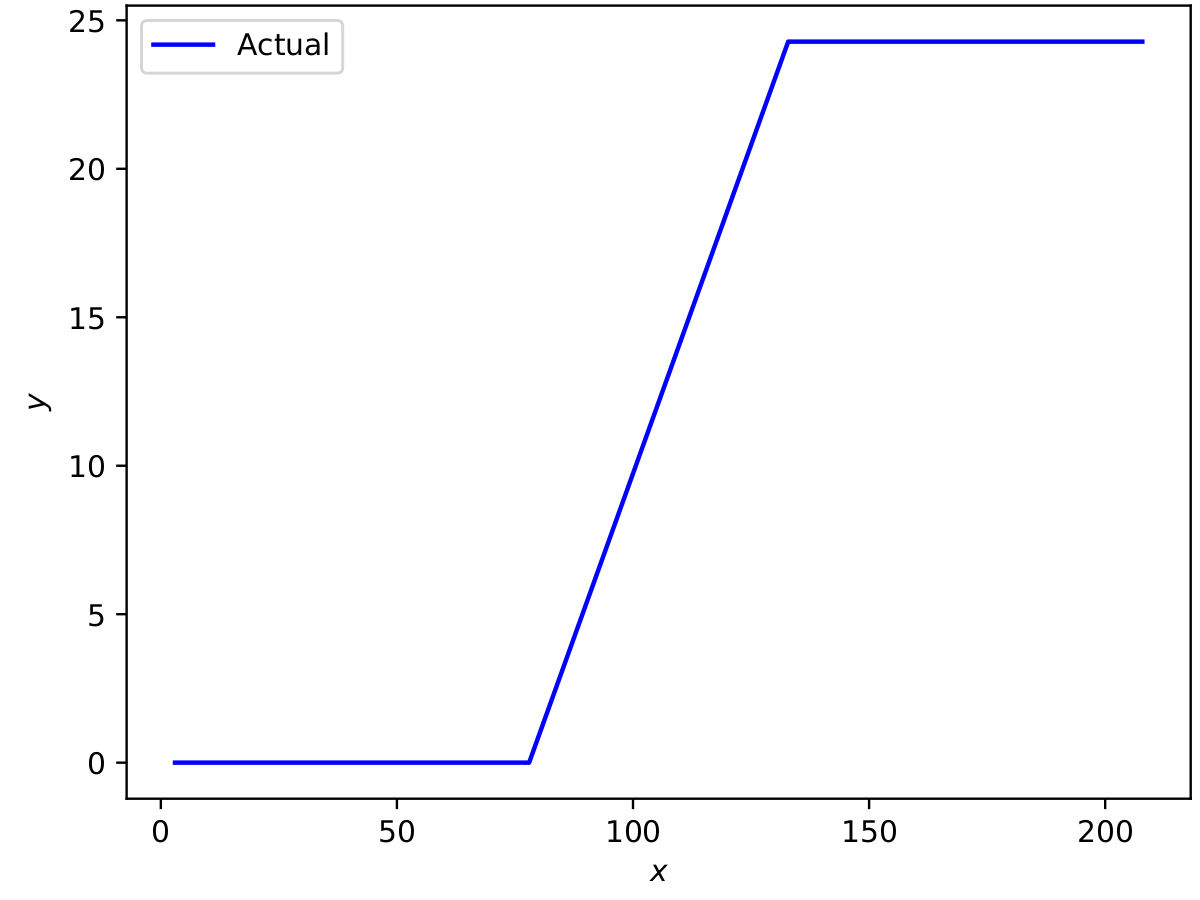
\includegraphics[scale=0.75]{problem17_4a_pure}
    \caption{Robot Planned Path}
    \label{fig:p17_4a_planned}
\end{figure}

\begin{figure}[h]
    \centering
    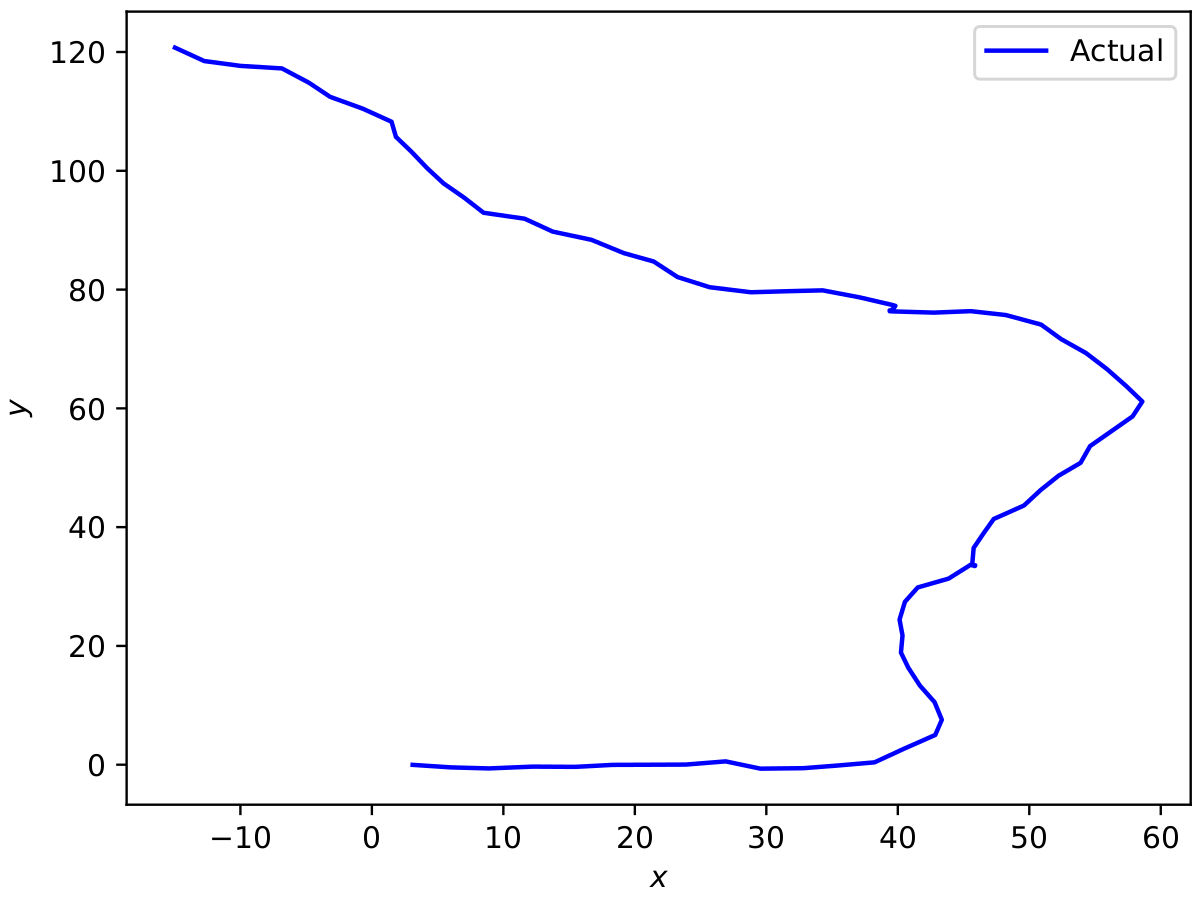
\includegraphics[scale=0.75]{problem17_4a_Vnoise_bad}
    \caption[Robot Planned Path (bad)]{Robot planned path when V is applied}
    \label{fig:p17_4a_vnoise_bad}
\end{figure}

\begin{figure}[h]
    \centering
    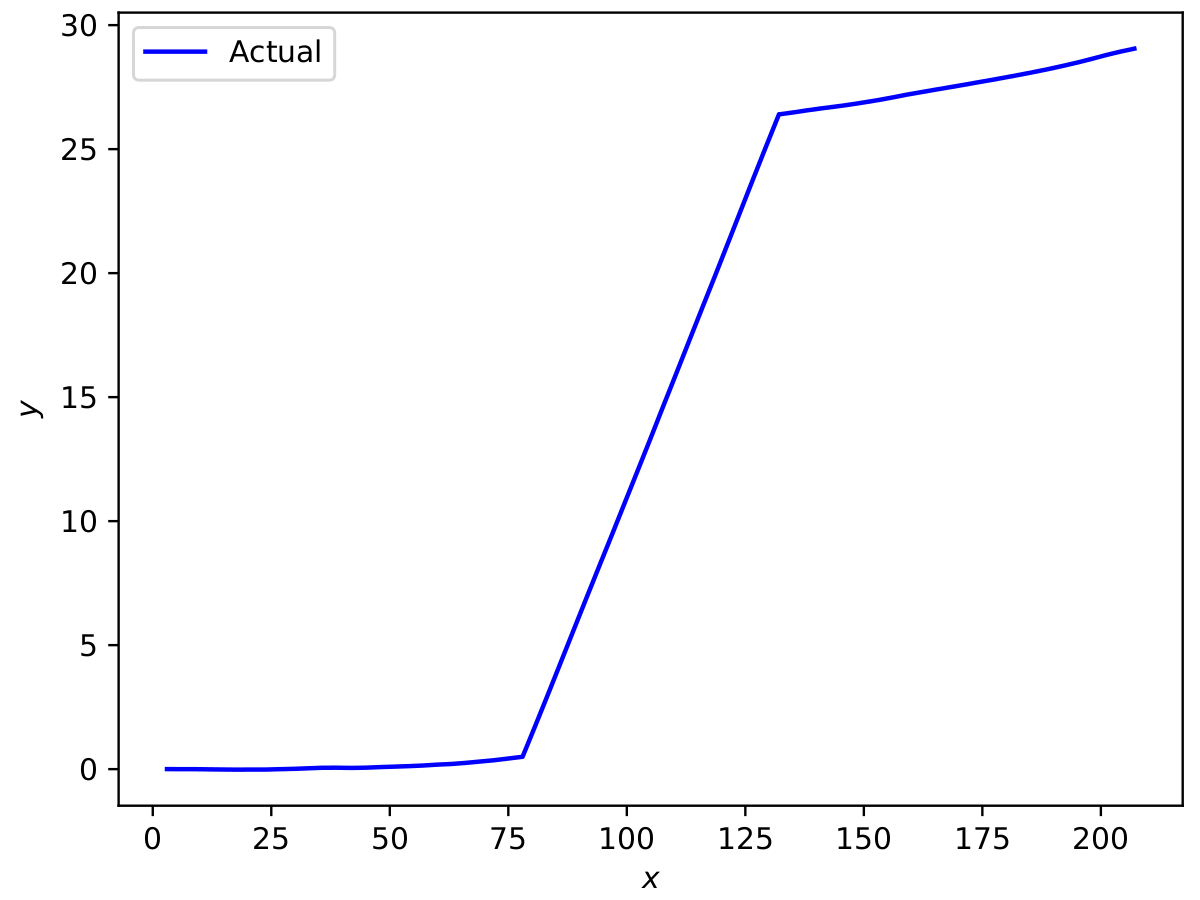
\includegraphics[scale=0.75]{problem17_4a_Vnoise_good}
    \caption[Robot Planned Path (good)]{Robot planned path when V is divided by 100}
    \label{fig:p17_4a_vnoise_good}
\end{figure}

\subsubsection{Problem 4b}
The basic Differential Drive equations can be discretized for application 
towards the EKF as follows:

$$f1 = x_{k+1} = x_k + \frac{r\Delta t}{2}\(\omega_{1, k} + \omega_{2, k})cos(\theta_k)$$
$$f2 = y_{k+1} = y_k + \frac{r\Delta t}{2}(\omega_{1, k} + \omega_{2, k})sin(\theta_k)$$
$$f3 = \theta_{k+1} = \theta_k + \frac{r\Delta t}{2}(\omega_{1, k} - \omega_{2, k})$$

Then take the partial derivatives to get Equation \hyperref[eq:F]{\textit{F}}.

\begin{equation}{\label{eq:F}}
\[
F =
  \begin{bmatrix}
    1 & 0 & -\frac{r\Delta t}{2}(\omega_{1, k} + \omega_{2, k})sin(\theta_k) \\
    0 & 1 & \frac{r\Delta t}{2}(\omega_{1, k} + \omega_{2, k})cos(\theta_k) \\
    0 & 0 & 1
  \end{bmatrix}
\]
\end{equation}

We then apply the following 
\href{http://roboscience.org/book/html/AdvFiltering/ExtendedKalmanFilter.html}{sequence of steps}:

\begin{enumerate}
    \item $\^{x}_{k|k-1} = f(\^{x}_{k-1|k-1}, u_k)$
    \item $P_{k|k-1} = F_kP_{k-1|k-1}F^T_k + V_k$
    \item $K_k = P_{k|k-1}H^T_k(H_kP_{k|k-1}H^T_k + W_k)^{-1}$
    \item $\^{x}_{k|k} = \^{x}_{k|k-1} + K_k\big(z_k - h(\^{x}_{k|k-1})\big)$
    \item $P_{k|k} = (I - K_kH_k)P_{k|k-1}$
\end{enumerate}

My code follows those steps pretty much exactly. There are more efficient ways to code it but for this assignment it's good. There are EKF libraries out there if I need efficiency.


\subsubsection{Problem 4c}
When $V = V / 100$ we get the image in Figure \ref{fig:p17_4a_xy}, which is what I believe the intended image was here.

\begin{figure}[h]
    \centering
    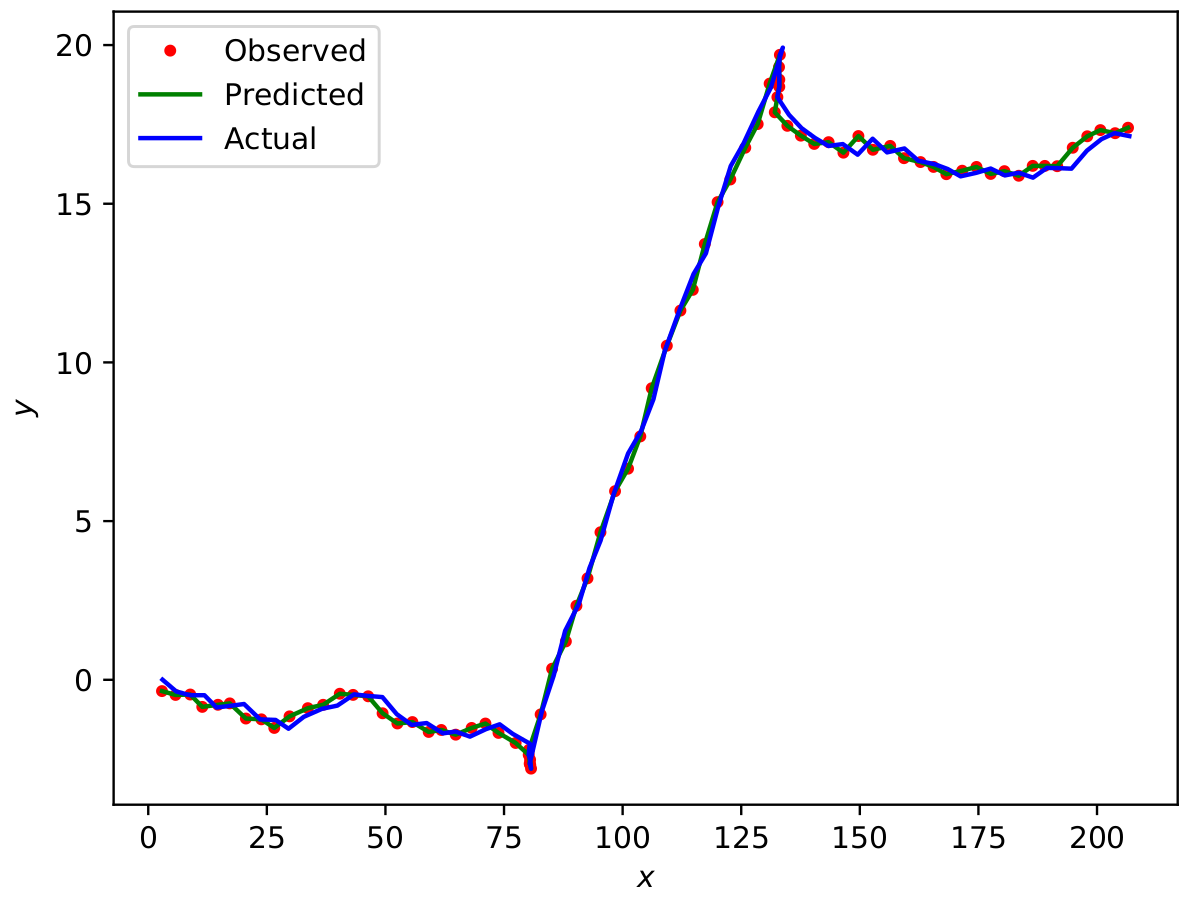
\includegraphics[scale=0.75]{problem17_4a_xy}
    \caption{Robot x-y positions}
    \label{fig:p17_4a_xy}
\end{figure}

\subsubsection{Problem 4d}
Figure \ref{fig:p17_4a_xyt} shows $x$-$y$ on the vertical axis and time on the 
horizontal axis.

\begin{figure}[h]
    \centering
    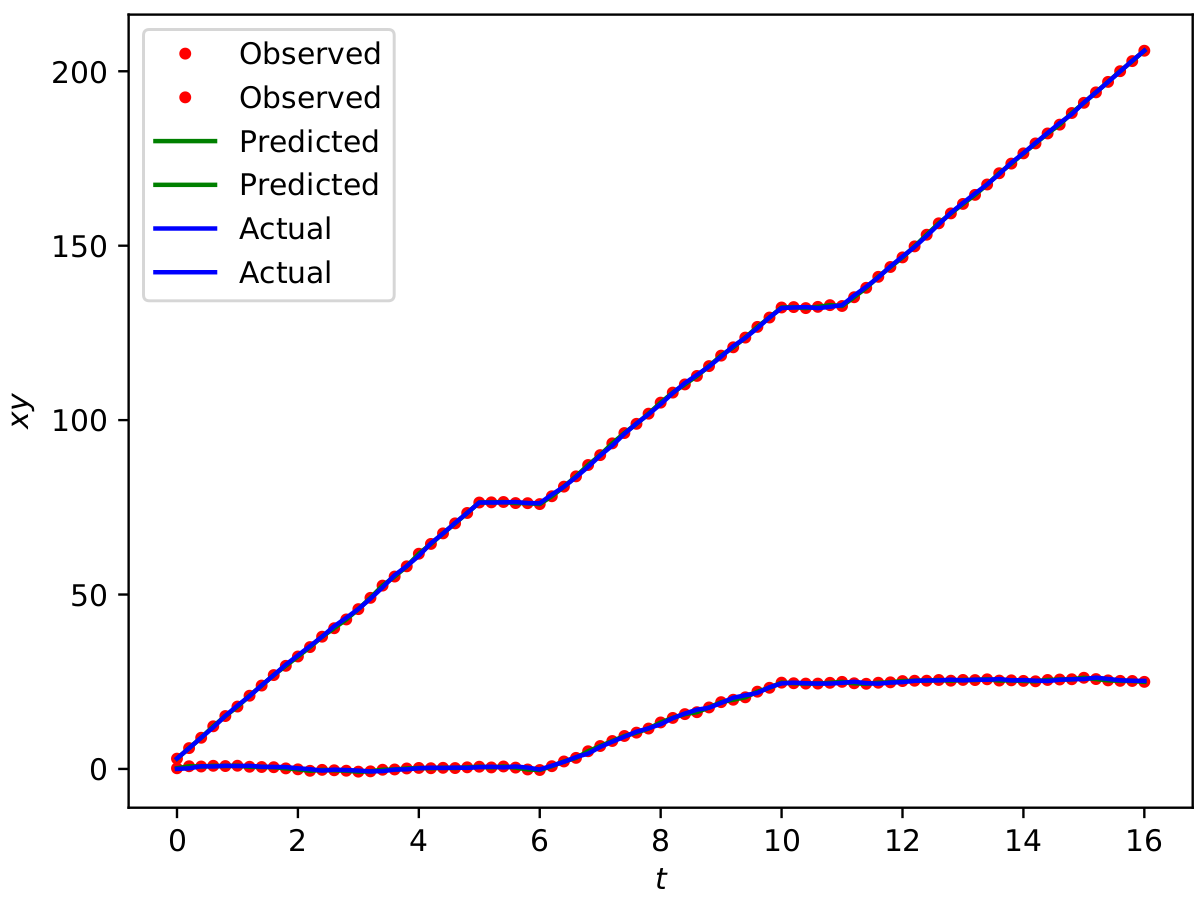
\includegraphics[scale=0.75]{problem17_4a_xy_t}
    \caption{Robot x-y over time}
    \label{fig:p17_4a_xyt}
\end{figure}

\subsubsection{Problem 4e}
Figure \ref{fig:p17_4a_ellipse} shows the ellipses on the filter. Something is 
slightly off with my filter so I threw a scaler at the ellispses so they would 
be visible. I used the same code from 17.3 with only minor modifications but 
something broke and I am out of time.

And on that note, the examples all use full $H$ matrices (observing all) whereas 
the homework problems utilized 1/2 and 2/3 sensor data which can lead to very 
messed up filters. You can't just pad it with zeros and I spend too long on 
this homework as is to track down what specifically causes this.

\begin{figure}[h]
    \centering
    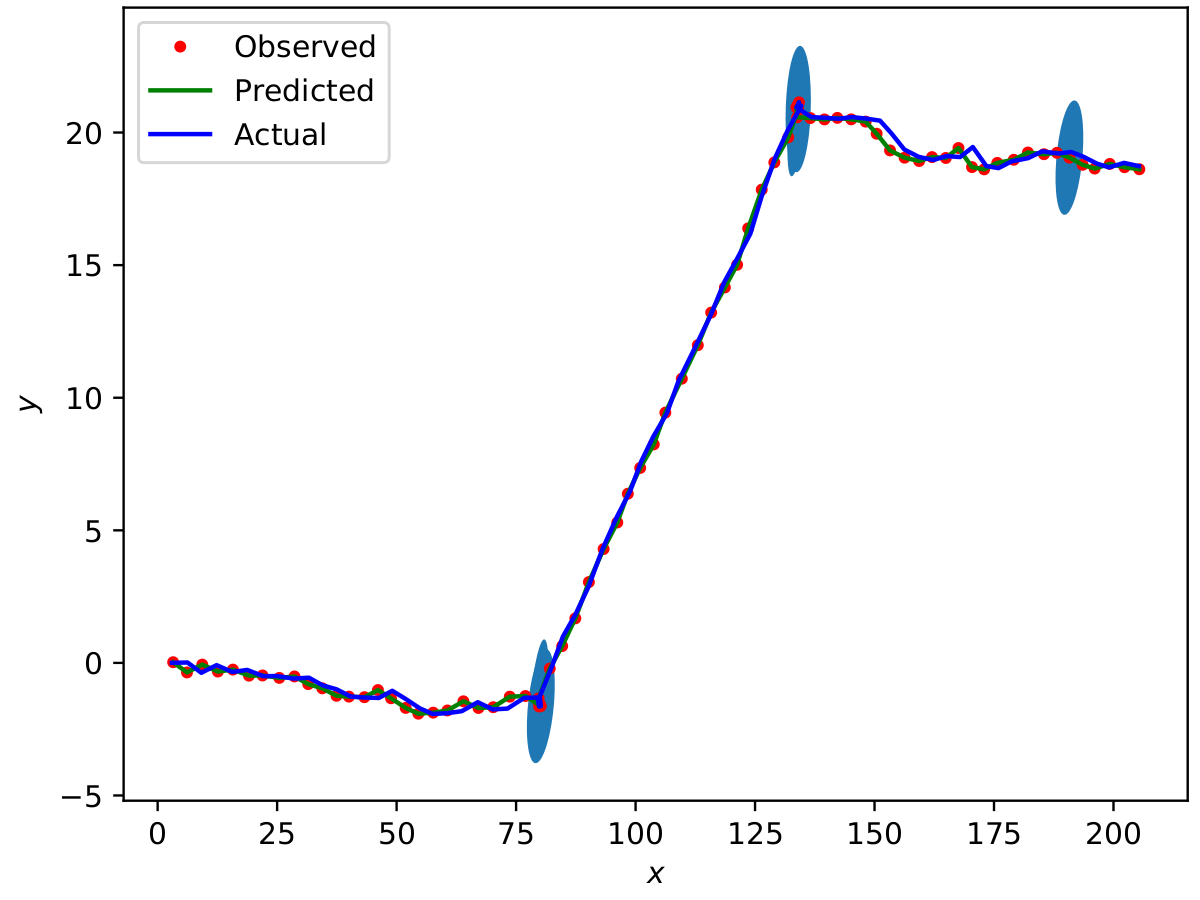
\includegraphics[scale=0.75]{problem17_4a_ellipse}
    \caption{Uncertainty Ellipses}
    \label{fig:p17_4a_ellipse}
\end{figure}


% \newpage
% \section{\textbf{Chapter 18}}
% \subsection{Problem 1}
% \subsubsection{Problem 1.1}
% asdf


% \subsubsection{Problem 1.2}
% asdf


% \subsubsection{Problem 1.3}
% asdf


\end{document}
